\section{\textbf{Simulation study}}

We utilize a simulation study to highlight the utility of AME as an inferential tool for dyadic analysis. The goal of the simulation is to assess how well AME can provide unbiased and well-calibrated estimates of coefficient parameters in the presence of unobserved dependencies. Specifically, we are concerned with conducting inference on regression parameters of a linear model for a network in the case where there is an omitted variable. For instance, assume that the true data-generating process for a particular $Y$ is given by:

\begin{align}
	y_{i,j} \sim  \mu + \beta x_{i,j} + \gamma w_{i,j} + \epsilon_{i,j}
	\label{eqn:sim}
\end{align}

where $Y= \{y_{i,j}\}\in \mathbb R^{n\times n}$ is an observed sociomatrix, $X = \{x_{i,j} \} \in \mathbb R^{n \times n}$ is a matrix of observed dyad-specific characteristics, and $W = \{ w_{i,j}\} \in \mathbb R^{n \times n}$ is a matrix of unobserved dyad-specific characteristics. $Y$ can be thought of as a dyadic dependent variable, $X$ and $W$ are both dyadic covariates that are a part of the data-generating process for $Y$, but $W$ is not observed. We compare inference for $\mu$ and $\beta$---the latter parameter would be of primarily theoretical concern for applied scholars---using three models :

\begin{itemize}
	\item the standard international relations approach assuming independent errors; 
	\item the AME approach outlined in the previous section with a unidimensional latent factor space ($K=1$);
	\item and an ``oracle'' regression model that assumes we have measured all sources of dependencies and thus includes both $x_{i,j}$ and $w_{i,j}$. 
\end{itemize}

The first model corresponds to the ``standard'' approach in which little is explicitly done to account for latent dependencies in dyadic data. In the second model, we account for dependencies in dyadic data using the AME framework described in the previous section. For both the first and second models, we are simply estimating a linear model of $X$ on $Y$, and assessing the extent to which inference on the regression parameters are complicated in the presence of unobserved dependencies, $W$. In the last model, we provide an illustration of the ideal case in which we have observed and measured $W$ and include it in our specification for $Y$. The oracle case provides an important benchmark for the standard and AME approaches.

For the simulation we set the true value of $\mu$ (the intercept term) to -2 and $\beta$ (the effect of $X$ on $Y$) to 1.\footnote{The value of $\gamma$ is also set to 1, which corresponds to a an example where the $W$ character is associated with homophily.} We conduct two sets of simulations, one in which the number of actors in the network is set to 50 and the other at 100. In total, we ran 1,000 simulations where we begin by simulating $Y$ from the specification given in Equation~\ref{eqn:sim} and then for each simulated $Y$ we estimated a standard, AME, and oracle model. 

We compare the performance of the models first in terms of how well they estimate the true values of $\mu$ and $\beta$ in Figure~\ref{fig:ameBias} by depicting the average $\mu$ and $\beta$ estimates from the simulations for the three models. The panels in the left show the results for when the number of actors is set to 50 and those on the right for 100; and the top pair of panels represents the estimates for $\mu$ while the bottom pair do the same for $\beta$. In each case, we find that the estimates for $\mu$ and $\beta$ produced by the standard approach are notably off from their true values. On the other hand, the AME model performs just as well as the oracle case in estimating the true values. 

\begin{figure}
	\centering
	\caption{Regression parameter estimates for the standard, AME, and oracle models from 1,000 simulations. Summary statistics are presented through a traditional box plot, and the estimates from each simulation are visualized as well as points.}
	\label{fig:ameBias}
	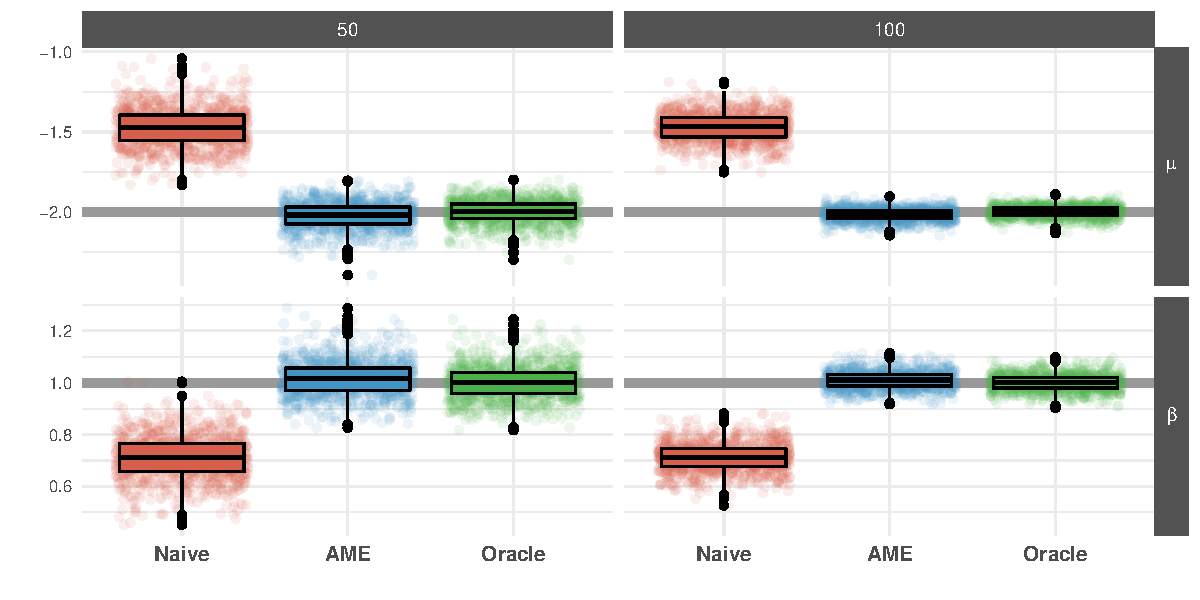
\includegraphics[width=1\textwidth]{ameSimBias_all.pdf} \\
\end{figure}

Next, we estimate the 95\% confidence interval for the three models in each of the simulations and estimate the proportion of times that the true value fell within those intervals. The results are summarized in Figure~\ref{fig:ameCalib}, and again we see that the AME approach performs as well as the oracle, while the standard approach performs poorly by comparison. 

\begin{figure}
	\centering
	\caption{Proportion of times the true value fell within the estimated 95\% confidence interval for the standard, AME, and oracle models from 1,000 simulations.}
	\label{fig:ameCalib}
	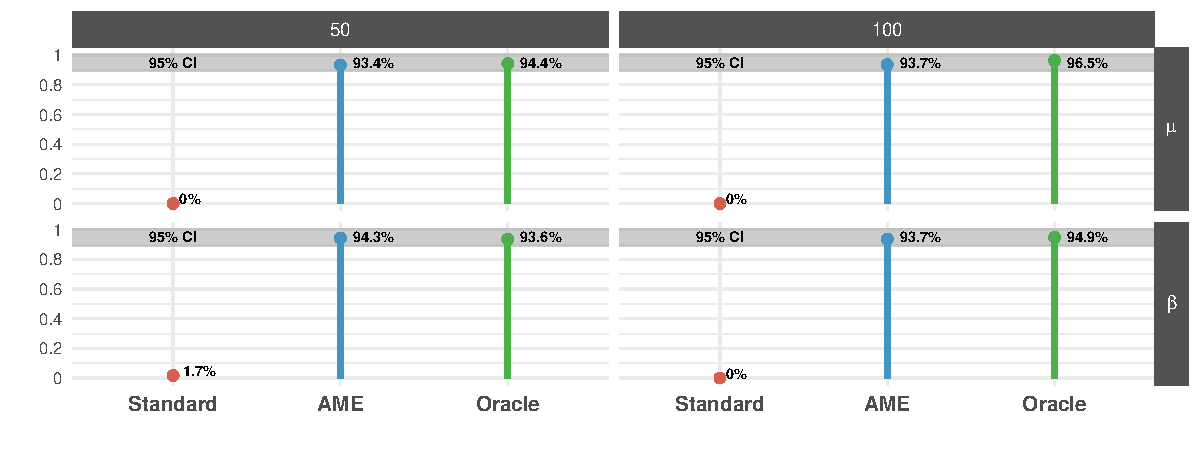
\includegraphics[width=1\textwidth]{ameSimCover_all.pdf} \\
\end{figure}

In the case of the data generating process for $Y$, $W$ is set as an unobserved dyadic covariate that had a homophilous effect on $Y$. Homophilous because $W$ within this framework is simply an example of a dyadic attribute involving $i$ and $j$ that positively affects the degree to which they will interact with one another, i.e., $y_{ij}$. This type of unobserved dependency will be captured through the multiplicative effects portion of the model, $\mathbf{U}^{\top} \mathbf{D} \mathbf{V}$. To estimate how well the model performs in doing this we recover the multiplicative effects term for each simulation and calculate the correlation between it and the unobserved dependency, $W$.\footnote{Specifically, since both the multiplicative effects term and $W$ are continuous dyadic variables, we calculate the Pearson correlation coefficient.} We visualize the distribution of the correlations from each of the 1,000 simulations in Figure~\ref{fig:ameCorr} for the case where the number of actors is set to 100 (top pair of panels) and 50. Additionally, we calculate the median across the correlations and display the result using a vertical line. For both $n=50$ and $n=100$, we find that the multiplicative effects perform very well in capturing the unobserved dependency, which indicates that the structure provided by this framework is not simply capturing noise but can be used as a tool to estimate unobserved structure. 

\begin{figure}
	\centering
	\caption{Distribution of correlation between missing variable and multiplicative random effect in AME across the 1,000 simulations. Vertical line through the distribution represents the median value across the simulations.}
	\label{fig:ameCorr}
	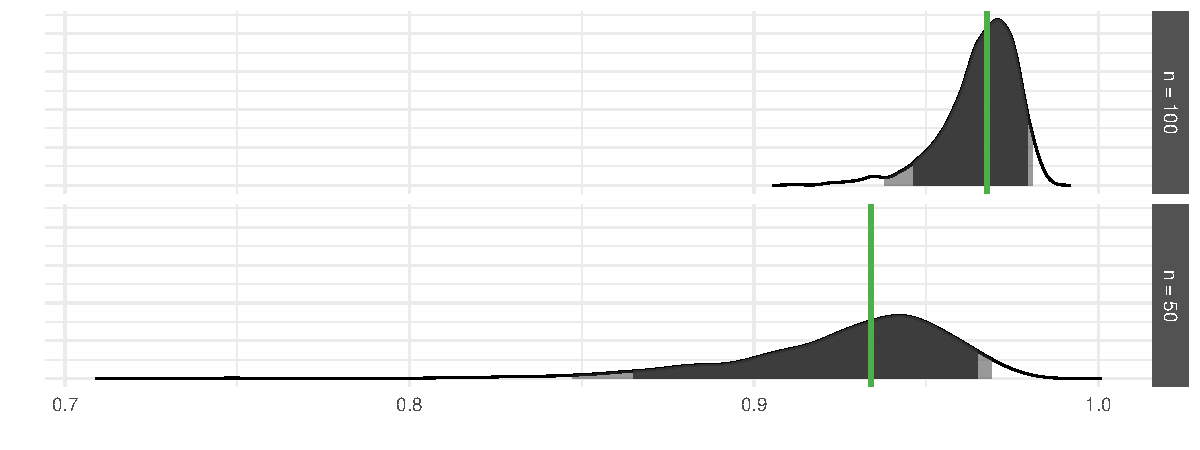
\includegraphics[width=1\textwidth]{ameSimCorr.pdf} \\
\end{figure}

What this simulation has shown is that beyond obtaining less biased and better-calibrated parameter estimates, a key benefit of the AME framework is that we can also estimate unobserved dependencies through the random effects structure of the model. 

% - in the presence of deendencies, ame can be used to easily perform accurate inference on exogenous parameters. the simulation here shows that the typial glm estimator has issues with bias and calibration
% - apart from just allowing inference on xbeta, the random effects are not just capturing random noise but underlying structure that we can further explore. we illustrate some strategies for doing so in teh application section. 